\chapter{Methods}
In this chapter we review the basic implementation details of our ViDA framework.
We first demonstrate how we use Lucas-Kanade and Farneback optical flow algorithms
to reduce the feature space to only 6 25 bin features. With that feature space,
we the show how to accurately classify activities in the videos using support
vector machines and k nearest neighbors. Finally, we cover the details of distributing
this system over an elastic cloud architecture for scalability and flexibility
using Amazon Web Services (AWS).


\section{\label{subsection:comparison}Comparison of Methods}
We implemented the Lucas-Kanade method first in our research because in general,
performance is a concern and, as long as not too many features or
too few features are detected, the Lucas-Kanade algorithm will be faster
\cite{de2015choosing}. Despite this fact, we found that our classifier did
not perform as well on features extracted from the Lucas-Kanade method, as it
did using the Farneback method. As a result, most of the results in this thesis
have been calculated with Farneback optical flow unless otherwise specified.

\section{\label{section:feature_extraction}Feature Extraction from Optical Flow}
The \texttt{CalculateVectors} function in both Algorithm \ref{alg:lk_flow} and
\ref{alg:farneback} returns several dense matrices that represent the features
that we can extract from the optical flow output. These features are magnitude,
orientation, x direction and y direction of the optical flow features. These
are ultimately the features that we use to train and classify using an SVM. However,
if we had two $N \times M$ video frames as the input, we now have $4 \times N \times M$
features. Clearly we have not yet reduced the input feature space. Thus, based
on information that we know \textit{a-priori}, we can reduce our feature space
significantly.

In the case of typing and writing, we know we can expect there to be motion from
one frame to the next. We don't know by how much, but we do know that it is not
zero. Using this knowledge, we can then threshold the optical flow vectors that
we get back from Algorithms \ref{alg:lk_flow} and \ref{alg:farneback}. The
threshold value used was empirically calculated from doing multiple runs on the
AOLME videos. We found we got the best results by only retrieving
optical flow vectors with a magnitude greater than 75\% of the max value. The set
of Equations in \ref{eq:optical_threshold} illustrate this idea.

\begin{align}
  \label{eq:optical_threshold}
  \begin{split}
  \mathbf{V} &= (\mathbf{V_x}, \mathbf{V_y}) \\
  \mathbf{V_m} &=
  \begin{cases}
    1, & \text{if } \|\mathbf{V}\| \geq \max( \|\mathbf{V}\|) \times 0.25 \\
    0, & \text{otherwise}
  \end{cases}
  \end{split}
\end{align}

where $\mathbf{V_x}$ and $\mathbf{V_y}$ are the optical flow vectors in the
x and y directions respectively. $\mathbf{V_m}$ is the bit mask that is
then used to extract the subset of data from each of the dense matrices.

\begin{align}
  \label{eq:subset}
  \begin{split}
  \text{Let: } \\
  \|\mathbf{V\prime}\| &= \|\mathbf{V}\| \circ \mathbf{V_m}\\
  \mathbf{V_x\prime} &= \mathbf{V_x} \circ \mathbf{V_m}\\
  \mathbf{V_y\prime} &= \mathbf{V_y} \circ \mathbf{V_m}\\
  \mathbf{\Phi\prime} &= \mathbf{\Phi} \circ \mathbf{V_m}
\end{split}
\end{align}

Using the optical flow bitmask, $\mathbf{V_m}$, we can then extract features
from each one of our dense matrices using the Hadamard product as shown in
Equation \ref{eq:subset}, where $\|\mathbf{V\prime}\|,
\mathbf{V_x\prime},\mathbf{V_y\prime}, \mathbf{\Phi\prime}$ are subset matrices
for the magnitude, x and y direction and orientation respectively. We have now
reduced the feature space somewhat, but depending the size of the video and the
amount of entropy per frame pair, we could still have a significant amount of
data to process for classification.

In addition to extracting generic vectors from the video, we also add
geometrical centroids, blob orientation and background motion around the blobs
to the optical flow statistics being used for classification. We implement these
methods to attempt to leverage information that could be useful during
classification. In order to calculate the geometrical centroids and orientations
of each blob, we use some well known algorithms available in OpenCV,
\texttt{connectedComponentsWithStats} and \texttt{findContours}
\cite{itseez2015opencv}. \texttt{connectedComponentsWithStats} is a function
that allows us to compute the centroid for each blob of connected pixels. The
input to this function is our binary mask image, $\mathbf{V_m}$. Once we have
all the connected blobs, we can then calculate the orientation of each one of
those blobs using \texttt{findContours} in combination with with
\texttt{fitEllipse}. The full implementation of this algorithm is outlined in
Appendix \ref{ap:centroids}. The final step is to then dilate each blob, and
then calculate the optical flow statistics in the difference region. Appendix
\ref{ap:dilate}. Figure \ref{fig:orient_cent} illustrates the idea of acquiring
the centroid and orientation of the blobs from $\mathbf{V_m}$.

\begin{figure}[h]
  \label{fig:orient_cent}
  \centering
  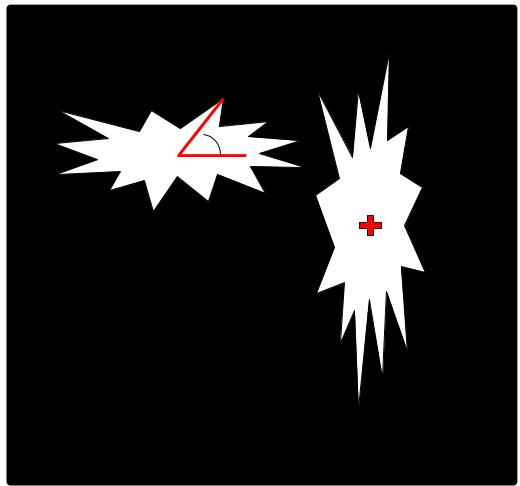
\includegraphics[width=8cm]{figures/cent_and_orient}
  \caption{Example of orientation measurement on the left, and the centroid calculation on the right.}
\end{figure}

When the previous optical flow features have been generated, their values are then
organized into a probability density function (PDF) with 25 bins. That is to say that
each frame pair generates a PDF and that PDF is accumulated for every subsequent
frame in the video sequence. When our software reaches the end of the video file,
a normalized, cumulative distribution function (CDF) is calculated and output
for each vector. So for each input video there will be one CDF with 25 bins
for blob orientation, blob centroid x and y, motion vector magnitude, motion
vector orientation and background motion vector magnitude. Figure \ref{fig:extract_flow}
clearly illustrates this concept.

\begin{figure}[h]
  \label{fig:extract_flow}
  \centering
  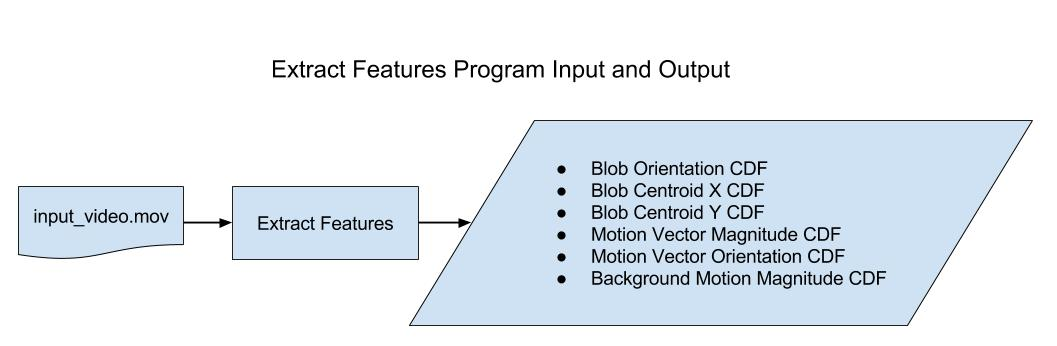
\includegraphics[width=14cm]{figures/extract_features_flow}
  \caption{Flow of the extract features program. For every input video, it will
  return a CDF with 25 bins for each of the extracted features from the motion
  vectors}
\end{figure}

\section{\label{section:the_data}The AOLME Dataset}
The AOLME dataset is an enormous repository of over 900 hours of video
recordings of students [reference needed]. The videos contain students
interacting with facilitators, their peers and computers to write code in
Python on the Raspberry Pi.  The dataset is wealth of information but difficult
to exploit in its current state.  The data used for this thesis is a subset of
the entire AOLME dataset. By hand, we have selected several videos and extracted
typing and writing clips from the original dataset and are using these as ground
truth for measuring the accuracy of our classification. Figure \ref{fig:typing_writing}
is representative of the features that have been extracted by hand.

\begin{figure}[h]
  \label{fig:typing_writing}
  \centering
  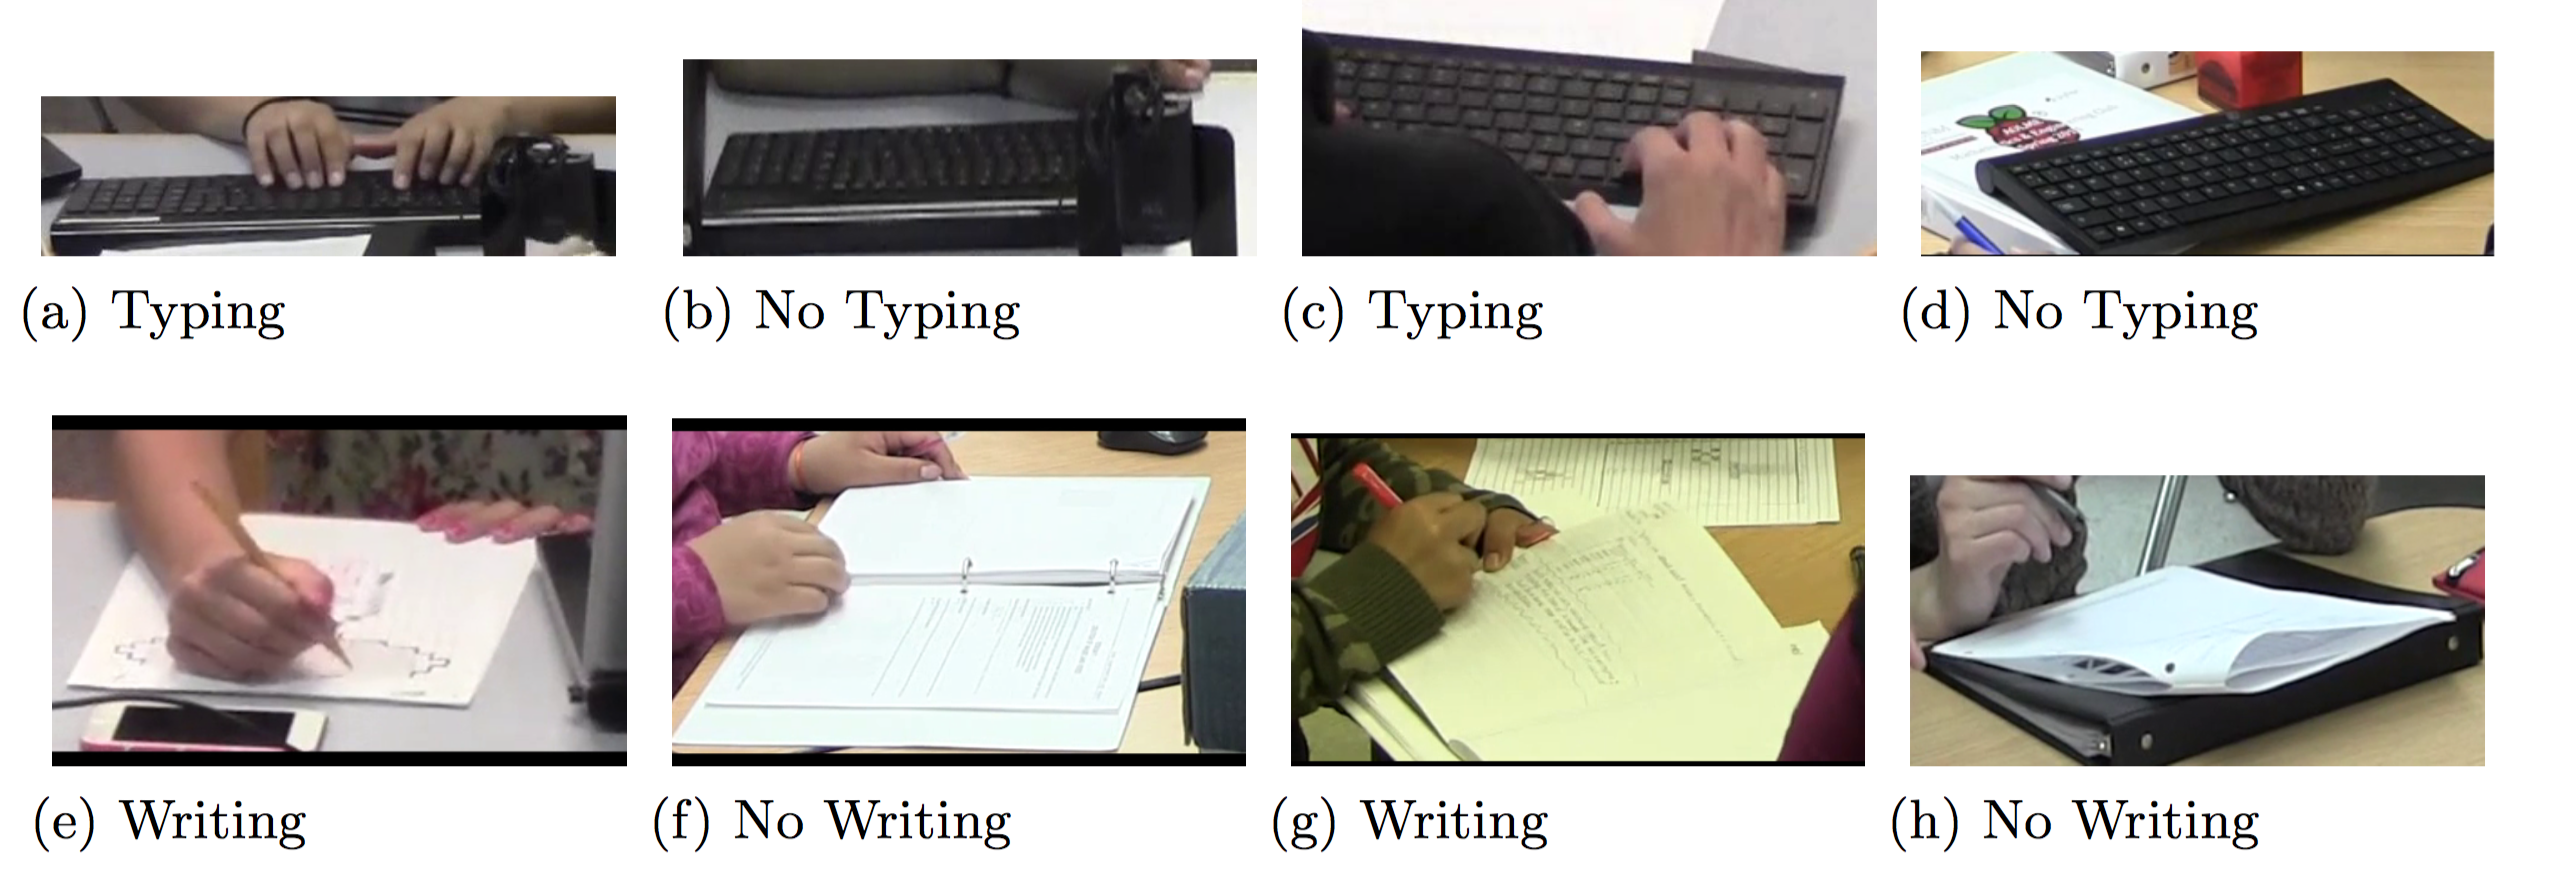
\includegraphics[width=\textwidth]{figures/typing_writing_clip}
  \caption{Example of features that have been manually extracted from the dataset
  for training and testing. For the above example, we need to classifiers for each
  activity to determine if the activity is being performed, or it is not.}
\end{figure}

As Figure \ref{fig:typing_writing} suggests, we are only using a cropped version
of the video. The reason for this is that we are not attempting to solve the tracking
problem in this thesis, only the classification problem. Hence, we assume that
the videos entering into our software have already been clipped and cropped with
the target activities inside of them and the corresponding lack of the activity.
Our subset of the AOLME database consists of the following:

\begin{itemize}
\item Twenty videos of typing
\item Twenty videos of no typing
\item Twenty videos of writing
\item Twenty Videos of no writing
\end{itemize}

\section{\label{section:classification}Classifying the Reduced Feature Space}
